\documentclass{xmgr}
\usepackage{ gensymb }
\usepackage{listings}
\usepackage[table]{xcolor}
\lstset{language=C}
\setcounter{secnumdepth}{5}
\usepackage{paralist}
\definecolor{orange}{rgb}{1,0.5,0}

\makeatletter
\newcommand\footnoteref[1]{\protected@xdef\@thefnmark{\ref{#1}}\@footnotemark}
\makeatother

\author   {Daniel Sienkiewicz}
\nralbumu {206358}
\email    {daniel@sienkiewicz.ovh}


\title    {Projekt komputera samochodowego bazujący na systemie mikrokomputera Intel Galileo}
\date     {2015}
\miejsce  {Gdańsk}

\opiekun  {dr inż. Janusz Młodzianowski}

\begin{document}

\begin{abstract}
Celem pracy jest stworzenie komputera pokładowego do samochodu, w którego skład wchodzi: \begin{enumerate}
\item Mikrokomputer Intel Galileo Gen 1, 
\item Ekran dotykowy FTDI EVE VM800B, 
\item Oprogramowanie,
\end{enumerate}

\end{abstract}
\keywords{Intel Galileo, 
 $I^2C$,
 SPI, 
 C, 
 Arduino,
 GPIO,
 FTDI EVE,
 VM800}
\maketitle

%================WPROWADZENIE=====================
\chapter{Wprowadzenie}
\section{Cele}
Celem pracy jest budowa oraz oprogramowanie komputera pokładowego do samochodu. Komputer powinien móc wczytać z czujników temperaturę panującą w silniku, na zewnątrz oraz w środku samochodu. Ponadto powinien on móc zapisać aktualną pozycję \emph{GPS} na karcie pamięci microSD oraz umożliwić korzystanie z kamerki cofania lub inteligentnego lusterka wstecznego. Komunikacja użytkownika z komputerem będzie odbywała się poprzez użycie ekranu dotykowego \emph{FTDI EVE VM800B}.
\section{Założenia}
Do wykonania komputera wykorzystano: \emph{Intel Galileo GEN 1} wraz z zainstalowanym oprogramowaniem \emph{Linux YOCTO}, \emph{Arduino IDE}, lokalizator \emph{GPS} służący do podawania aktualnej pozycji dzięki której obliczana zostaje droga przebyta przez samochód, kamerka internetowa służąca jako czujnik cofania oraz inteligentne lusterko wsteczne oraz symulator samochodu. Aktualnie komputer nie będzie zamontowany do fizycznego samochodu więc do tych celów zbudowany został symulator składający się z podstawowych czujników takich jak: guziki służące za czujnik zapięcia pasów/zamknięcia drzwi, potencjometry służące za czujniki temperatury oraz \emph{I/O expander PCF8574N} pozwalający na komunikację z \emph{Intel Galileo}. Na komputerze nie będzie wyświetlana aktualna prędkość ani przebieg ponieważ nawet w najnowszych samochodach nie jest to dostępna opcja. Dane te są dostępne na zegarach samochodowych więc nie ma potrzeby powtarzania tej informacji.

\section{Plan pracy}
Pierwszy rozdział opisuje podstawowe cele oraz założenia projektu.

Druga część pracy przedstawia architekturę projektu wraz z jego opisem funkcjonalnym. Opisuję również mechanizmy komunikacji systemu mikroprocesorowego z otoczeniem. Do komunikacji pomiędzy urządzeniami zostały wykorzystane 2 podstawowe protokoły komunikacyjne: \emph{$I^2C$} oraz \emph{SPI}.

W następnym rozdziale przedstawiony zostaje pomysł implementacji oraz proces tworzenia niezbędnej do obsługi symulatora samochodu biblioteki pozwalającej na komunikację poprzez \emph{I/O Expander PCF8574N} z \emph{Intel Galielo}. Zostaje tutaj również opisany proces tworzenia oprogramowania ekranu dotykowego \emph{FTDI EVE VM800B} wraz z biblioteką niezbędą do komunikacji pomiędzy Galileo i ekranem.

Ostatnia część pracy przedstawia pomysły  możliwych rozszerzeń projektu o dodatkowe moduły oraz funkcjonalności w zależności od potrzeb użytkownika.
%================KONIEC WPROWADZENIE=====================

%================ARCHITEKTURA=====================
\chapter{Architektura}
\subsection{Mechanizmy komunikacji systemu mikroprocesorowego z otoczeniem}
\subsubsection{Porty}

Porty są jednym z najbardziej podstawowych interfejsów. Najczęściej dzieli się je na porty:
\begin{enumerate}
	\item Cyfrowe
	\item Analogowe
\end{enumerate}

Porty cyfrowe charakteryzują się możliwością przyjęcia lub wysłania sygnału binarnego (1 - jest sygnał, 0 - sygnału nie ma). Najczęściej wysłanie sygnału równego 1 jest równoznaczne z wysłaniem napięcia o wartości 5V oraz odpowiednio wysłanie 0 jest równoznaczne z wysłaniem napięcia równego 0V. Z kolei porty analogowe mogą przesyłać sygnały nawet 10 bitowe. Każdy z portów może działać w jednym  z dwóch trybów: wejścia - oczekiwać na przyjęcie danych od urządzenia zewnętrznego oraz wyjścia - wysyłać dane do urządzenia zewnętrznego.

W środowisku Arduino aby obsłużyć port analogowy wystarczy ustaliś tryb w jakim ma on działać (wejście/wyjście) a następnie wysłać/odczytać dane. Dla portu analogowego wygląda to następująco:
\begin{lstlisting}[label=bot-dirs-alg,caption=Obsługa portu analogowego w środowisku Arduino]
int val = 0;
int analogPin = A1;	
pinMode(analogPin, OUTPUT);
val = analogRead(analogPin);
pinMode(analogPin, INPUT);
analogWrite(ledPin, val);
\end{lstlisting}

oraz odpowiednio dla portu cyfrowego:
\begin{lstlisting}[label=bot-dirs-alg,caption=Obsługa portu cyfrowego w środowisku Arduino]
int val = 0;
int digitalPin = 1;	
pinMode(digitalgPin, OUTPUT);
val = digitalRead(analogPin);
pinMode(digitalPin, INPUT);
digitalWrite(digitalPin, HIGH);
\end{lstlisting}

W środowisku linux każdy z portów możemy traktować jako plik, więc wpisanie lub odczytanie danych z portu jest równoznaczne z odpowiednio wpisaniem lub odczytaniem danych z pliku. Komunikację z portem możemy prowadzić w dowolnym języku. Dla języka C wygląda to następująco:

\begin{lstlisting}[label=bot-dirs-alg,caption=Obsługa portu cyfrowego w środowisku Linux (język C)]
FILE *fp;
int value;

// Ustawienie portu cyfrowego nr 13 jako port wyjścia
fp = fopen("/sys/class/gpio/gpio39/direction", "w");
fprintf(fp, "out");
fclose(fp);

// Wpisanie wartości do portu cyfrowego
fp = fopen("/sys/class/gpio/gpio39/value", "w");
fprintf(fp, "1");
fclose(fp);

// Odczytanie wartości z portu cyfrowego
fp = fopen("/sys/class/gpio/gpio39/value", "r");
fscanf(fp, "%i", &value);
fclose(fp);
\end{lstlisting}

oraz podobnie dla języków skryptowych np. Bash:

\begin{lstlisting}[label=bot-dirs-alg,caption=Obsługa portu cyfrowego w środowisku Linux (bash)]
# Ustawienie portu cyfrowego nr 13 jako port wyjścia
root@henio:~# echo -n "out" > /sys/class/gpio/gpio39/direction

# Wpisanie wartości do portu cyfrowego
root@henio:~#  echo -n "0" > /sys/class/gpio/gpio39/value
root@henio:~#  echo -n "1" > /sys/class/gpio/gpio39/value

# Odczytanie wartości z portu cyfrowego
root@henio:~# echo -n "in" > /sys/class/gpio/gpio28/direction
root@henio:~# cat /sys/class/gpio/gpio28/value
\end{lstlisting}

Przy komunikacji należy jednak pamiętać, że w Galileo nazwy urządzeń nie są intuicyjne tzn. port IO4 nie jest plikiem /sys/class/gpio/gpio4.

\subsubsection{Przerwania}

Przerwania są to bezpośrednie funkcje systemu lub sprzętu ułatwiające komunikację ze światem zewnętrznym. Część z nich jest zarezerwowana przez system lecz część jest wolna do wykorzystania przez programistę. Przerwania możemy podzielić na trzy podstawowe rodzaje:

\begin{enumerate}
	\item Programowe
	\item Sprzętowe
	\begin{enumerate}
		\item Niemaskowalne (NMI\footnote{Non-Maskable Interrupt})
		\item Maskowalne
	\end{enumerate}
	\item Wyjątek
\end{enumerate}

Przerwania programowe wywołuje się za pomocą komendy \emph{INT XX}, gdzie \emph{XX} oznacza numer przerwania zadeklarowanego w tablicy wektorów przerwań\footnote{ang. interrupt vector table - tablica zawierająca adresy podprogramów służących do obsługi wektorów przerwań}, która jest tworzona przy każdorazowym starcie systemu. Przerwanie to może przyjąć wartości do 255 i są one zarezerwowane przez procesor oraz użytkownika.

Przerwanie sprzętowe jest to rodzaj przerwań wywoływanych przez urządzenia wejścia/wyjścia lub zgłaszane przez procesor. Zostają one wywołane niezależnie w określonych przypadkach. Przerwania te dzielimy na maskowalne oraz niemaskowalne. Główna różnica między nimi polega na możliwości zablokowania przerwań maskowalnych podczas gdy przerwania niemaskowalne muszą zostać obsłużone. Przykładem przerwania niemaskowalnego jest \emph{INT2} czyli popularny \emph{Blue Screen of Death}\footnote{Ekran błędu w systemach Windows pojawiający się po krytycznym błędzie systemu}.

Ostatnim rodzajem przerwań są wyjątki. Wywoływane są podczas napotkania przez procesor błędów oraz niepowodzeń. Arduino oczywiście obsługuje przerwania. Ich obsłga jest bardzo prosta. W środowisku Arduino aby obsłużyć port analogowy wystarczy wysołąć funkcję \emph{attachInterrupt}:

\begin{lstlisting}[label=bot-dirs-alg,caption=Obsługa przerwań sprzętowych w środowisku Arduino]
attachInterrupt(pinInt, funcName, mode);
\end{lstlisting}
gdzie \emph{pinInt} jest to pin na którym Arduino będzie nasłuchiwało na przerwanie, \emph{funcName} jest to nazwa funkcji, która zostanie wykonana gdy przerwanie zostanie zgłoszone, \emph{mode} jest to określenie kiedy sygnał może być uznany za przerwanie. \emph{Mode} może przyjmować wartości: 
\begin{enumerate}
	\item LOW - przerwanie zostanie zgłoszone gdy wartość na określonym pinie jest równa LOW\footnote{Wartość w środowisku arduino równoznaczna z napięciem 0V na określonym pinie}
	\item CHANGE - przerwanie zostanie zgłoszone gdy wartość na określonym pinie zostanie zmieniona
	\item RISING - przerwanie zostanie zgłoszone gdy wartość na określonym pinie zostanie zmieniona z LOW na HIGH\footnote{Wartość w środowisku arduino równoznaczna z napięciem 5V na określonym pinie}
	\item FALLING - przerwanie zostanie zgłoszone gdy wartość na określonym pinie zostanie zmieniona z HIGH na LOW
\end{enumerate}

\subsubsection{Odpytywanie w pętli}
Jednym z najprostszych metod pozyskania danych z mikro kontrolera jest jego odpytywanie w nieskończonej pętli. Jest to najmniej efektywny sposób ponieważ cały czas zajmuje niepotrzebnie zasoby sprzętu niepotrzebnymi zapytaniami.

\begin{lstlisting}[label=bot-dirs-alg,caption=Odpytywanie w nieskończonej pętli w środowisku Arduino]
void loop() {
	funcName();
	delay(1000);
}
\end{lstlisting}

Funkcja \emph{loop()} jest równoznaczna z funkcją \emph{main()} w języku C, z tą różnicą, że jest wykonywana od momentu startu (zaraz po jednorazowym wykonaniu funkcji \emph{setup()} ) aż do wyłączenia systemu. Taką sytuację można utożsamiać sobie z wywołaniem jakiejkolwiek funkcji w bloku \emph{while(1)}.

\subsubsection{Timer}
Kolejnym sposobem na komunikację z mikro kontrolerem (lub systemem operacyjnym) jest użycie dostępnego Timera. Polega to na wywołaniu funkcji co określony czas, którego zarządzaniem zajmuje się urządzenie (lub system operacyjny). Rozwiązanie to jest bardzo podobne do odpytywania w pętli, a następnie wywołania funkcji \emph{delete()} z tą różnicą, że użycie timera jest dokładniejsze ponieważ wykorzystuje zegar czasu rzeczywistego znajdującego się w CPU\footnote{ang. Central Processing Unit - jednostka arytmetyczno-logiczna wykorzystywana do wykonywania obliczeń niezbędnych do działania programu}.
\begin{lstlisting}[label=bot-dirs-alg,caption=Przykładowe użycie timer w środowisku Arduino]
#include <TimerOne.h>
Timer1.initialize(500000);
Timer1.attachInterrupt(funcName, 500000);
\end{lstlisting}

%================KONIEC ARCHITEKTURA=====================

%================IMPLEMENTACJA=====================
\chapter{Implementacja}
\subsection{Intel Galileo}
Intel Galileo jest  to mikro kontroler oparty na 32-bitowym procesorze Intel® Quark SoC X1000 i taktowaniu 400MHz. Został on wyposażony w 14 pinów cyfrowych (w tym 6 pinów mogących pełnić funkcję \emph{PWM}\footnote{ang. Pulse-Width Modulation - technika pozyskiwania wyników analogowych poprzez użycie wyjść cyfrowych}) oraz 6 pinów cyfrowych. Każdy z tych pinów jest w stanie operować napięciem od 0V do max 5V. Bardzo dużym atutem Galileo jest wbudowana karta sieciowa, port RS-232, port USB oraz slot karty microSD. Galileo może być używane w dwóch trybach - trybie w pełni kompatybilnym z Arduino oraz w trybie z zainstalowanym systemem operacyjnym (np. Linux).\cite{GalileoBook}

\begin{figure}[!h]
    \centering
    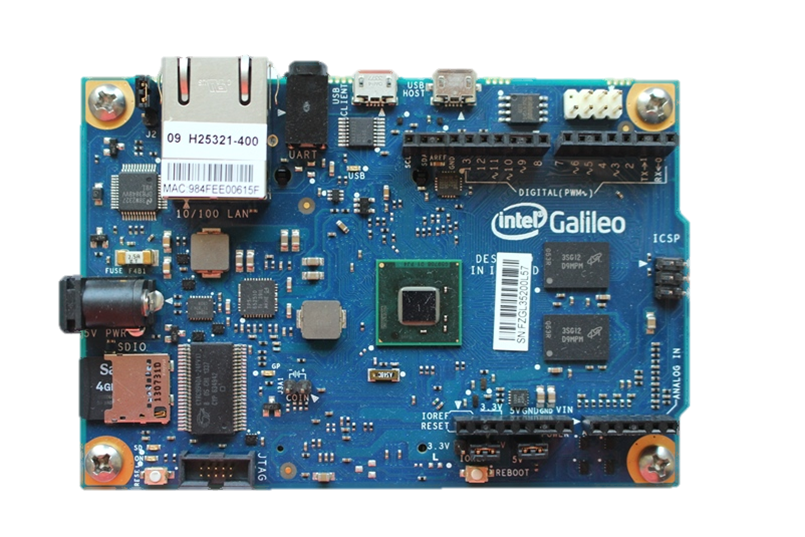
\includegraphics[height=0.4\textwidth]{images/galileo.png}
    \caption{Galileo Gen 1 Board \label{Galileo Gen 1 Board}}
    \source{\url{http://www.intel.com/content/www/us/en/embedded/products/galileo/galileo-g1-datasheet.html}\cite{GalileoBoard}}
\end{figure}

\begin{figure}[!h]
    \centering
    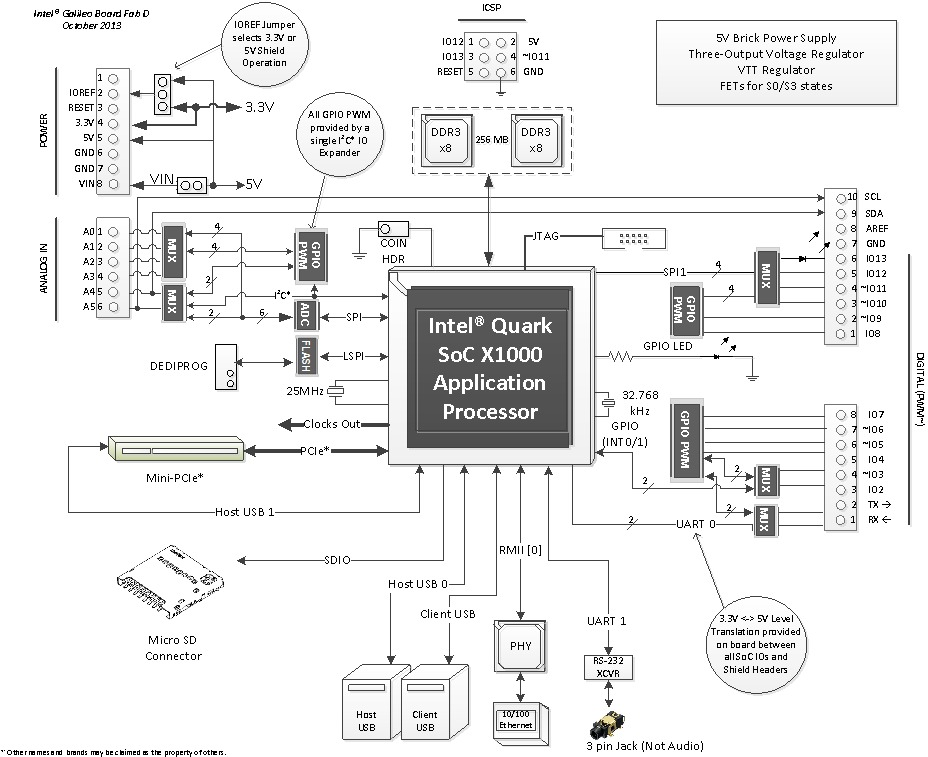
\includegraphics[height=0.8\textwidth]{images/IntelGalileoLogicSchematics.jpg}
    \caption{Schemat logiczny układu Intel Galileo\label{IntelGalileoLogicSchematics}}
    \source{\url{https://www.arduino.cc/en/ArduinoCertified/IntelGalileo}\cite{IntelGalileo}}
\end{figure}

Do komunikacji z Galileo programista może użyć portu RS-232, USB (działające w trybie host oraz client) oraz wyjścia Ehernet. Intel Galileo jest zasilane napięciem 5V i 2.0A, które może być dostarczone poprzez zasilacz dostarczony do zestawu lub poprzez podłączenie zasilania do portów PWR\footnote{Port używany jako port zasilania(5V)} oraz GND\footnote{Port używany jako masa}. Najprostszym sposobem na uruchomienie programu jest skompilowanie go za pomocą środowiska Arduino Studio, pisząc w języku C i używając dostarczonych przez producenta Arduino funkcji do obsługi portów, a następnie przesłania skompilowanej wersji poprzez kabel USB do urządzenia. Po przesłaniu program zostaje automatycznie uruchomiony. Gdy mamy zainstalowany system operacyjny wtedy komunikację można prowadzić w dowolnym języku programowania.

\section{Protokół komunikacyjny $I^2C$}
\emph{$I^2C$}\footnote{ang. Inter-Integrated Circuit} jest szeregowym interfejsem stworzonym przez firmę \emph{Philips} służącym do przesyłania danych między urządzeniami elektrycznymi. 

Podstawową cechą \emph{$I^2C$} jest wykorzystywanie dwóch linii służących do komunikacji: dwukierunkowa linia \emph{SDA\footnote{ang. Serial Data Line}} oraz jednokierunkowa linia \emph{SCL\footnote{ang. Serial Clock Time}}. Każdą transmisję danych należy rozpocząć sygnałem \emph{START} oraz zakończyć sygnałem \emph{STOP}. Dane wysyłane są od najstarszego do najmłodszego bitu oraz otrzymanie każdego z nich musi być potwierdzone przez odbiornik (bit ACK\footnote{ang. Acknowledge}). Należy również pamiętać, aby każdą komunikację z urządzeniem rozpocząć i zakończyć ustawiając linie \emph{SDA} oraz \emph{SCL} w stan nieaktywny (HIGH). Podstawowymi zaletami protokołu są:
\begin{enumerate}
	\item Połączenia składają się tylko z dwóch linii co znacznie ogranicza liczbę kabli wychodzących z urządzenia
	\item Duża dostępność sprzętu w sklepach
	\item Transmisja jest odporna na zakłócenia zewnętrzne
	\item Bez większych problemów można dodawać oraz odejmować układy korzystające z magistrali
\end{enumerate}

Nazwa $I^2C$ jest nazwą zastrzeżoną dlatego też w literaturze bardzo często spotyka się określenie \emph{TWI}\footnote{ang. Two Wire Interface}. Jest ono stosowane w mikro kontrolerach firmy \emph{Atmel}. 

\begin{figure}[!h]
    \centering
    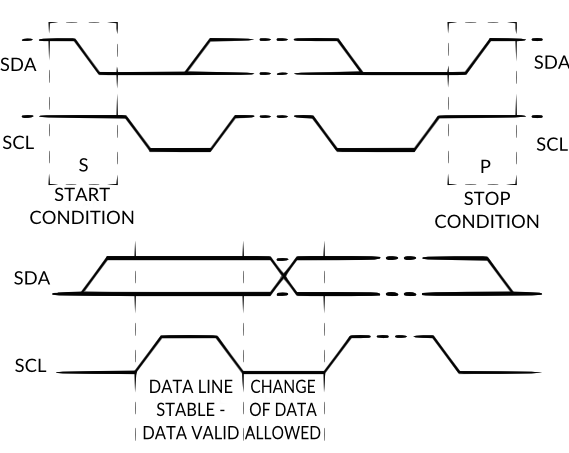
\includegraphics[height=0.3\textheight]{images/i2c.png}
    \caption{Przebieg czasowy protokołu $I^2C$}
    \source{\url{http://www.byteparadigm.com/applications/introduction-to-i2c-and-spi-protocols/}\cite{byteparadigm}}
\end{figure}

\subsection{Użycie protokołu $I^2C$ na przykładzie I/O Expander PCF8574N}
Odbieranie danych rozpoczyna się wysłaniem sygnału \emph{START}, a następnie zaadresowaniu urządzenia. Kolejnym krokiem jest ustalenie trybu (w tym wypadku \emph{READ}) oraz odczytanie potwierdzenia. Po wykonaniu tych czynności można rozpocząć odbieranie danych, które należy zakończyć wysłaniem sygnału \emph{STOP}.

Wygenerowanie sygnału \emph{START} polega na ustawieniu linii \emph{SDA} oraz \emph{SCL} w stan niski (LOW), a wygenerowanie sygnału \emph{STOP} polega na ustawieniu linii \emph{SDA} oraz \emph{SCL} w stan wysoki (HIGH).

Adresowanie urządzenia odbywa się poprzez wysłanie pojedynczych bitów adresu (pamiętając o kolejności MSB->LCB\footnote{Wysyłanie odbywa się w kolejności od najbardziej znaczących (najstarszych) bitów}) oraz wygenerowanie impulsu zegara. Gdy chcemy zaadresować urządzenie, którego adresem jest np. 4 należy wykonać:
\begin{lstlisting}[label=bot-dirs-alg,caption=Adresowanie urządzenia $I^2C$ na przykładzie PCF8574N]
for(m = 0x80; m; m >>= 1){
    if(adres & m)         
      digitalWrite(sda, HIGH);
    else
      digitalWrite(sda, LOW);
        
   digitalWrite(scl, HIGH);
   digitalWrite(scl, LOW); 
}
\end{lstlisting}
Po otrzymaniu potwierdzenia na linii \emph{SDA} można zacząć czytać dane przesyłane z urządzenia.

\begin{figure}[!h]
    \centering
    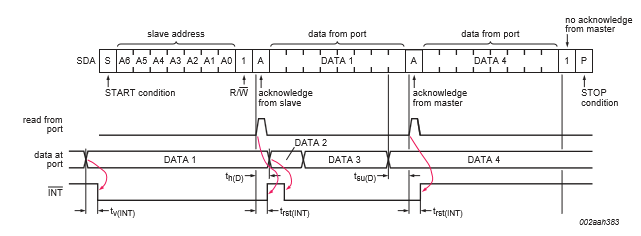
\includegraphics[height=0.25\textheight]{images/read_i2c.png}
    \caption{Przykładowy schemat odbierania danych poprzez $I^2C$ na przykładzie PCF8574N\label{$I^2C$}}
    \source{Karta katalogowa I/O Expander PCF8574N}
\end{figure}

Podobnie jak odbieranie danych, wysyłanie danych należy rozpocząć od wysłania sygnału \emph{START} wraz z adresem urządzenia oraz trybem (\emph{WRITE}). Po otrzymaniu potwierdzenia można rozpocząć wysyłanie danych w odpowiednich dla urządzenia paczkach x-bitowych. Po wysłaniu każdej z nich otrzymamy potwierdzenie. Na zakończenia transmisji należy wysłać sygnał \emph{STOP}.

\begin{figure}[!h]
    \centering
    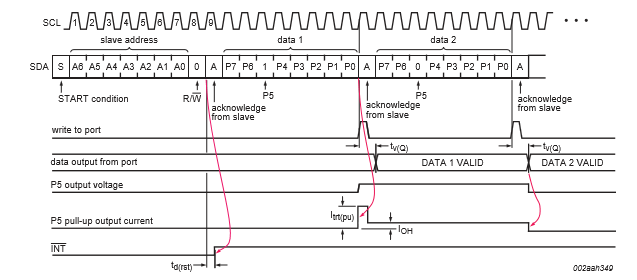
\includegraphics[height=0.2\textheight]{images/write_i2c.png}
    \caption{Przykładowy schemat wysyłania danych poprzez $I^2C$ na przykładzie PCF8574N\label{$I^2C$}}
    \source{Karta katalogowa I/O Expander PCF8574N}
\end{figure}

\subsection{Problemy z bibliotekami}
\subsection{Własna implementacja $I^2C$}
\subsection{Własna biblioteka do komunikacji poprzez $I^2C$ dla Intel Galileo}

\section{Protokół komunikacyjny SPI}
Kolejnym przykładem interfejsu szeregowego jest protokół SPI\footnote{ang. Serial Peripherial Interface}. Składa się on z czterech podstawowych linii - dwóch służących do przesyłania danych w przeciwnych kierunkach, jednej z sygnałem taktującym synchronizującym transfer danych oraz linii chip select. 

Linia MISO\footnote{ang. Master In Slave Out} jest linią wejścia danych dla urządzenia nadrzędnego (master), a wyjściem dla urządzenia podrzędnego (slave), linia MOSI\footnote{ang. Master Out Slave In} jest wyjściem dla urządzenia master, a wejściem dla slave. Linia SCK\footnote{ang. Serial Clock} jest wejściem taktującym zegar. Sygnał taktujący jest zawsze generowany przez układ master. Transmisja danych na obydwu liniach jest zawsze dwukierunkowa i odbywa się jednocześnie - nadanie danych na linii MISO wiąże się z nadaniem danych na linii MOSI. Nie zawsze jednak nadane dane niosą ze sobą informację - najczęściej nadawane informacje płyną w jedną stronę podczas, gdy w tym samym czasie wysyłane zostają puste dane.\cite{Dorra}

\begin{figure}[!h]
    \centering
    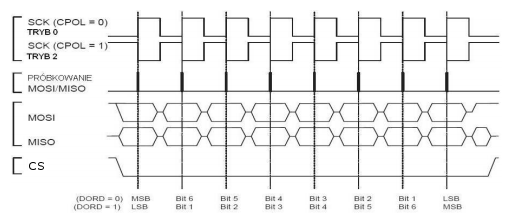
\includegraphics[height=0.25\textheight]{images/spi.png}
    \caption{Przebiegi czasowe interfejsu SPI dla sygnału zegarowego o CPHA=0}
    \source{\url{http://castor.am.gdynia.pl/~dorra}\cite{Dorra}}
\end{figure}

\subsection{Komunikacja poprzez protokół SPI}
Komunikacja zawsze przebiega dwustronnie (duplex\footnote{Nadawanie i odbieranie informacji odbywa się w obu kierunkach}). Zmienia taktu zegara z niskiego na wysoki daje możliwość odczytania danych z linii MISO i jednocześnie wysłania danych na linię MOSI. W przypadku zmiany taktu zegara z wysokiego na niski dane zostają wysłane poprzez linię MISO i jednocześnie odczytane z linii MOSI. W porównaniu z $I^2C$ protokół SPI jest dużo szybszy. Maksymalna prędkość protokółu $I^2C$ w wydaniu z 2012r. to 5-MHz, gdy prędkość SPI jest praktycznie nieograniczona.

\subsection{VM800B}
\emph{FDTI EVE VM800B} jest to wyświetlacz dotykowy wraz z wbudowanym kontrolerem audio. Podstawowe cechy urządzenia\cite{FTDI}:
\begin{enumerate}
	\item Pojedynczy układ scalony dla wyświetlacza oraz kontrolera Audio
	\item Ekran 3.5" LCD
	\item 262 tys. kolorów
	\item Możliwość wygładzania krawędzi
	\item Możliwość komunikacji poprzez użycie interfejsu $I^2C$ lub SPI
	\item Wbudowane widgety dostępne dla użytkownika
	\item Zakres pracy wyświetlacza: $-40^{\circ} C$ do $85^{\circ} C$ 
\end{enumerate}

Komunikacja Galileo z Ekranem odbywa się poprzez protokół komunikacyjny \emph{SPI}. DO tego celu została napisana własna wersja funkcji służących do wysłania oraz odczytania danych z ekranu.

\subsection{Symulator samochodu}
Do celów implementacjach komputer nie mógł zostać zamontowany do fizycznego samochodu. Do celów testowych zstał zabudowany symulator samochodu składający się z:
\begin{enumerate}
	\item 5 guzików symulujących drzwi samochodu (wraz z bagażnikiem)
	\item 4 guzików symulujący pasy pasażerów
	\item 3 potencjometrów symulujących czujniki temperatury w samochodzie
	\item 1 guzika symulującego wrzucenie biegu wstecznego
	\item 1 guzika symulującego włączenie świateł w samochodzie
\end{enumerate}
Guziki wysyłają sygnały cyfrowe, a potencjometry sygnały analogowe. Komunikacja z Galileo odbywa się poprzez użycie protokołu $I^2C$ wykorzystywane poprzez \emph{I/O Expander PCF 8574N} oraz 3 linii wyprowadzonych dla sygnałów analogowych.

%SCHEMAT LOGICZNY KOMPUTERA POKŁADOWEGO

\begin{figure}[!p]
    \centering
    	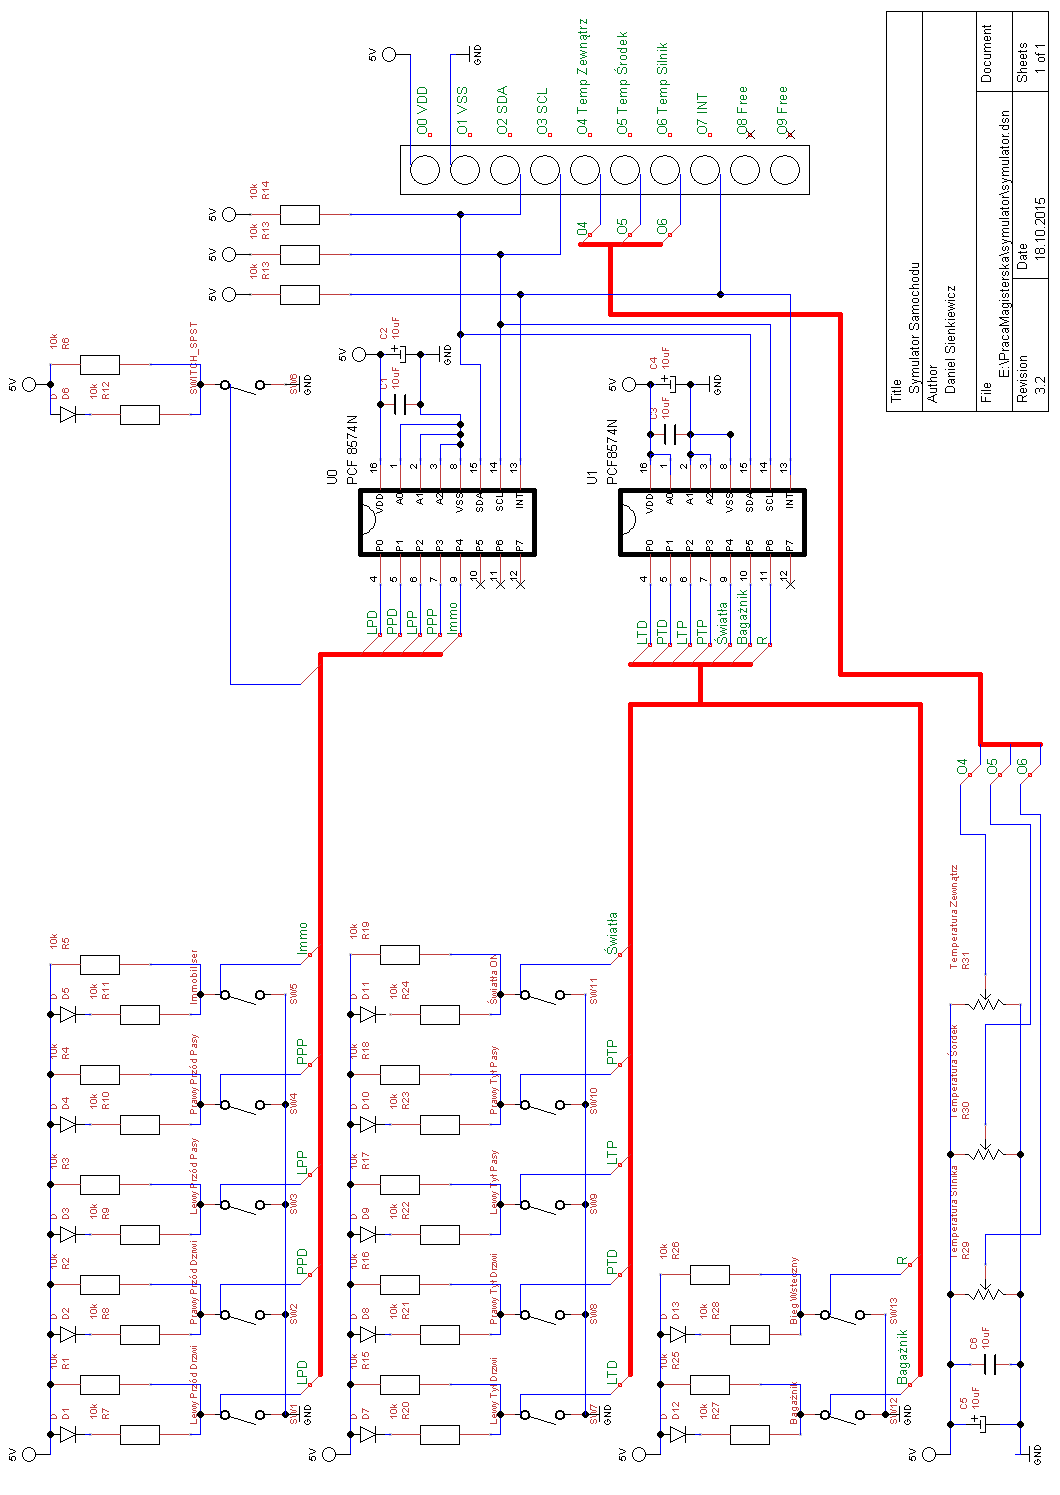
\includegraphics[height=0.9\textheight]{images/symulator.png}
    \caption{Schemat elektryczny symulatora samochodu}
    \source{Opracowanie własne}
\end{figure}
\chapter{Działanie komputera pokładowego}
\section{Założenia funkcjonalne projektu}
Najważniejszym założeniem funkcjonalnym była komunikacja z zestawem czujników, które mogą być zamontowane w samochodzie. W projekcie zostały użyte czujniki otwarcia/zamknięcia drzwi, zapięcia pasów, włączenia/wyłączenia świateł oraz czujniki temperatury. Dodatkowym elementem była komunikacja z zewnętrznym ekranem dotykowym służącym do komunikacji pomiędzy użytkownikiem a komputerem.

\section{Opis działania}
Proponowany komputer pokładowy jest całkowicie osobnym systemem niezależnym od sprzętu aktualnie posiadanego w samochodzie. Użytkownik po wejściu do samochodu oraz włączeniu zapłonu powoduje automatyczny start systemu. Na ekranie pojawia się powitanie oraz ekran startowy, na którym można zobaczyć aktualną pozycję GPS, temperaturę panującą w środku samochodu, na zewnątrz oraz w silniku. Stan drzwi i pasów zwizualizowany został poprzez miniaturkę samochodu z aktywnie otwierającymi się drzwiami, zapalającymi światłami oraz ikonką obrazującą stan zapiętych pasów. Na ekranie widnieją 2 przyciski - \emph{Save data} oraz \emph{Smart Mirror}. Pierwszy z nich daje możliwość zapisu aktualnej pozycji GPS oraz temperatur na karcie pamięci microSD, drugi przechodzi w tryb aktywnego lusterka wstecznego, który może również służyć jako czujnik cofania co bardzo przydaje się podczas parkowania w ciasnych miejskich parkingach. Wyłączenie systemu następuje wraz z wyłączeniem zapłonu w samochodzie.

\section{Dalsze kroki oraz propozycje}
Komputer został tak zaprojektowany tak aby w łatwy sposób można było dodać kolejne funkcjonalności zależne od potrzeb użytkownika. Jako propozycje można uwzględnić:
\begin{enumerate}
	\item Czujnik deszczu - automatyczne włączenie wycieraczek i dopasowanie ich prędkości w zależności od obfitości opadów i prędkości samochodu, dodatkowe włączenie wycieraczki tylnej w momencie gdy zostanie wrzucony bieg wsteczny
	\item Sterowanie głośnością radia w zależności od prędkości samochodu
	\item Blokada immobilizer
	\item Obsługa telefonu komórkowego za pomocą bluetooth
	\item Router - dodanie modułu karty WiFi w połączeniu z odbieraniem sieci komórkowej GPRS oraz rozsyłanie jej w samochodzie
\end{enumerate}
Jednak na potrzeby tej wersji projektu nie zostały one zaimplementowane. Oczywiście ogranicza nas tylko nasza wyobraźnia oraz finanse jakie chcemy przeznaczyć na rozbudowę systemu o dodatkowe moduły. 
%================KONIEC IMPLEMENTACJA=====================

\summary
TO DO

\appendix
\chapter{Karty Katalogowe}
Katalog \emph{datasheets} zawiera karty katalogowe użytych podzespołów
\begin{enumerate} 
\item Intel Galileo.pdf - Karta katalogowa Intel Galileo
\item PCF8574.pdf - Karta katalogowa I/O Expander PCF 8574N
\item VM800B.pdf - Karta katalogowa ekranu FTDI EVE VM800B
\end{enumerate}
\chapter{Porównanie dostępnych na rynku mikro kontrolerów}
\begin{table}[!tbh]
\begin{tabular}{|c|c|c|c|} \hline
 & \textbf{Intel Galileo} & \textbf{Raspberry Pi (Model B)} & \textbf{Arduino Uno} \\ \hline
Wymiary & 10cm x 7cm & 85.60mm x 56mm x 21mm & 5.59cm x 16.5cm \\ \hline
Procesor & Intel Quark X1000 & Broadcom BCM2835 & ATmega328 \\ \hline
Taktowanie & 400MHz	& 700MHziv & 16 MHz\\ \hline
Cache & 16 KB & 32KB L1 cache, 128KB L2 cache & - \\ \hline
RAM & 512 SRAM & 512 SRAM & 2 kB \\ \hline
Analog I/O	& 6 & 17 & 6 \\ \hline
Digital I/O	& 14 & 8 & 14 \\ \hline
PWM	& 6 & 1 & 6 \\ \hline
\end{tabular}
\caption{Specyfikacja dostępnych na rynku mikro kontrolerów}
\source{\url{http://eu.mouser.com/applications/open-source-hardware-galileo-pi/}\cite{GalileoVSRaspberry}}
\source{\url{http://botland.com.pl/arduino-moduly-glowne/1060-arduino-uno-r3.html}\cite{Botland}}
\end{table}

\chapter{Mapowanie portów Intel Galileo na pliki w systemie Linux}
\begin{table}[!hp]
\begin{tabular}{|c|c|c|} \hline
\textbf{Quark X1000} & \textbf{Sysfs GPIO} & \textbf{Galileo/Arduino port} \\ \hline
GPORT4 BIT7 & gpio51 & IO1 \\ \hline
GPIO6 & gpio14 & IO2 \\ \hline
GPIO7 & gpio15 & IO3 \\ \hline
GPORT1 BIT4 & gpio28 & IO4 \\ \hline
GPORT0 BIT1 & gpio17 & IO5 \\ \hline
GPORT1 BIT0 & gpio24 & IO6 \\ \hline
GPORT1 BIT3 & gpio27 & IO7 \\ \hline
GPORT1 BIT2 & gpio26 & IO8 \\ \hline
GPORT0 BIT3 & gpio19 & IO9 \\ \hline
GPORT0 BIT0 & gpio16 & IO10 \\ \hline
GPORT1 BIT1 & gpio25 & IO11 \\ \hline
GPORT3 BIT2 & gpio38 & IO12 \\ \hline
GPORT3 BIT3 & gpio39 & IO13 \\ \hline
GPORT4 BIT0 & gpio44 & A0 \\ \hline
GPORT4 BIT1 & gpio45 & A1 \\ \hline
GPORT4 BIT2 & gpio46 & A2 \\ \hline
GPORT4 BIT3 & gpio47 & A3 \\ \hline
GPORT4 BIT4 & gpio48 & A4 \\ \hline
GPORT4 BIT5 & gpio49 & A5 \\ \hline
\end{tabular}
\caption{Mapowanie portów Intel Galileo na pliki w systemie Linux}
\source{\url{http://www.malinov.com/Home/sergey-s-blog}\cite{SergeySBlog}}
\end{table}

\chapter{Programy}
Katalogi \emph{Galileo, PCF8574N} zawierają kod źródłowy oprogramowania stworzonego na potrzeby pracy. 

\noindent Katalog \emph{Galileo} zawiera oprogramowanie mikrokomputera Intel Galileo.

\noindent Katalog \emph{PCF8574N} zawiera oprogramowanie I/O Expander PCF8574N.

\bibliographystyle{unsrt}
\bibliography{magisterka}

\listoftables

\listoffigures

\oswiadczenie

\end{document}